\section{Objectives}
Cover uncompensated Lab 5.A and Miller/RC-compensated Lab 5.B from \textit{AIC Lab.pdf}, PDF pages 48--58, with frequency, DC and transient measurements. The model library is supplied separately by the user. The 1.0 V supply is a teaching adaptation, not a certification of the model voltage rating. Numerical plots for the handout's original 3.3 V process are not used directly as pass thresholds. The circuits are rebuilt from the handout topology; the earlier code is used only to review dimensions and omissions.

\section{Specification Mapping}
S denotes actual simulation and D derivation/discussion. PM<45 means the original capacitor case misses the handout recommendation of 45 degrees.
\small\begin{longtable}{p{.46\linewidth}p{.30\linewidth}p{.15\linewidth}}\toprule
Requirement and PDF pages & Deck / check & Status \\ \midrule\endhead
Two-stage open-loop gain and phase (48--50) & D01 & S+D \\
Uncompensated buffer and PM interpretation (50--51) & D01/C0,D05/C0 & S+D \\
2 pF and series-R compensation (52--54) & D01,D05/C1--2 & S+D; PM<45 \\
Low-frequency gain, -3dB, unity and PM (54) & D01; 10pF adaptation & S+D \\
ICMR and inverting -10 output swing (54--55) & D03--04 & S+D \\
CMRR, PSRR+ and PSRR- (56--57) & D02 & S+D \\
Both slew directions and settling (58) & D05 & S+D \\
\bottomrule\end{longtable}\normalsize


\section{Circuit and Design Derivation}
\[
 |A_0|\simeq\frac{g_{m2}}{g_{ds2}+g_{ds4}}\,
 \frac{g_{m7}}{g_{ds7}+g_{ds8}},\qquad
 \mathrm{PM}=180^\circ+\angle A(j2\pi f_u),\quad |A(j2\pi f_u)|=1.
 \]
 \[
 R_z\simeq1/g_{m7},\qquad
 |A(f_{3dB})|=|A(1\,\mathrm{Hz})|/\sqrt2,\qquad
 SR_{20-80}=\frac{0.6|\Delta V_o|}{t_{80}-t_{20}}.
 \]The circuit uses $I_{ref}=10\,\mu$A and $L=0.3\,\mu$m. Widths of M1/M2, M3/M4, M5, M6, M7 and M8 are 35, 54, 2.2, 30, 269 and 73 $\mu$m. The primary load is 10 pF, with 1 pF separately compared. A calibrated small DC differential offset centers open-loop output near 0.5 V without an added AC servo. Actual operating-point derivatives estimate stage gains of 101.03 and 90.25, whose product 9118 approximates the measured 9088.

The uncompensated baseline approximates an open capacitor with $10^{-21}$ F. C1 uses 2 pF; C2 uses 2 pF + 330 $\Omega$; C3 explicitly adapts to 10 pF + 330 $\Omega$; C4 retains that compensation with a 1 pF load. Actual $1/g_{m7}\approx187.74\,\Omega$, so 330 $\Omega$ is not exact zero cancellation. The page 48 first-stage denominator has device indices inconsistent with its schematic; M2/M4 at the first-stage output are used here.

\section{Simulation Setup}
Runs use PrimeSim HSPICE S-2021.09 win64, a baseline temperature of 27 $^\circ$C, \texttt{runlvl=5}, \texttt{accurate}, and \texttt{.op/.print/.measure} outputs. Every \texttt{.alter} resets all baseline parameters and temperature to prevent state from carrying into the next case. Actual runs completed without an error or failed measurement. Suppressed model warnings remain, so a warning-free run is not claimed. Public netlists contain no model paths. This comment marks the model setup required locally before execution; the model and its configuration remain local:
\begin{verbatim}
* MODEL_SETUP_REQUIRED
\end{verbatim}
CSV files and numerical summaries are in the lab's \texttt{results/} directory. Every figure is redrawn from actual printed data, not a waveform-viewer screenshot. \texttt{manifest.json} supplies specification mapping and case definitions.Five decks contain 19 cases. AC uses 1 Hz--10 GHz and 80 points/decade, with unwrapped phase and the first descending unity crossing. The buffer sweeps 0--1 V in 1 mV steps. The inverting circuit uses 10 k$\Omega$/100 k$\Omega$ input/feedback resistors and a 0.65 V reference, giving ideal $V_o=7.15-10V_{in}$; input sweeps 0.55--0.75 V in 0.2 mV steps. Valid tracking means at most 10 mV absolute error. Steps use 0.60--0.75 V, 1 ns edges, 1 $\mu$s delay, 5 $\mu$s observation and at most 0.2 ns steps. Settling requires all remaining samples to stay within 1\% of the measured final step.

\section{Results and Specification Checks}
\begin{center}\small\begin{tabular}{lrrrr}\toprule
Case & $A_0$ (dB) & $f_{3dB}$ (kHz) & $f_u$ (MHz) & PM (deg) \\ \midrule
0 & 79.17 & 156.659 & 124.561 & -5.78 \\
1 & 79.17 & 10.718 & 63.272 & 25.10 \\
2 & 79.17 & 10.718 & 64.364 & 35.84 \\
3 & 79.17 & 2.269 & 20.295 & 80.59 \\
4 & 79.17 & 2.274 & 21.016 & 93.66 \\
\bottomrule\end{tabular}\end{center}

\begin{figure}[htbp]\centering
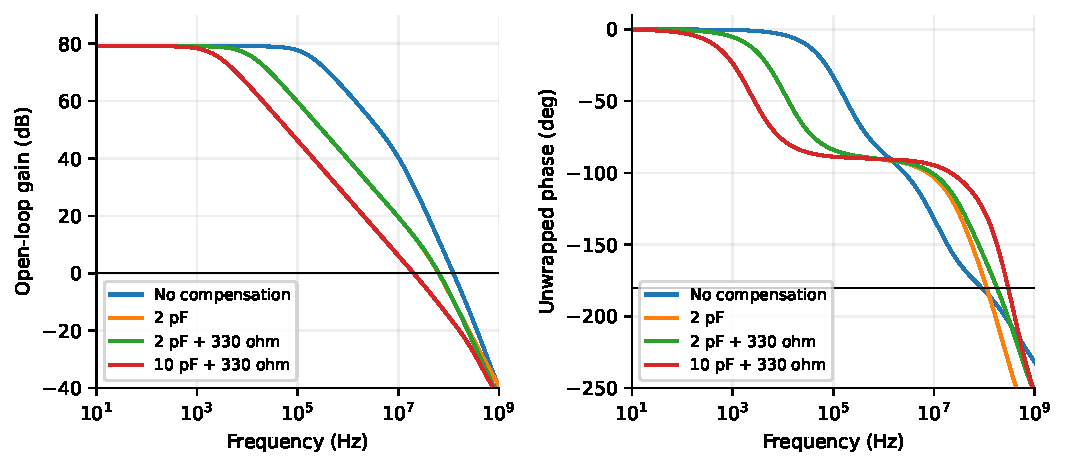
\includegraphics[width=\linewidth]{figures/compensation.pdf}
\caption{Open-loop gain and unwrapped phase. Both 2 pF and 2 pF + 330 ohms remain below 45 degrees under these adapted conditions.}
\end{figure}
Uncompensated gain is 79.17 dB with PM=-5.78 degrees. The 2 pF case reaches 25.10 degrees and series 330 $\Omega$ raises it to 35.84 degrees. At 10 pF, PM becomes 80.59 degrees while unity frequency drops to 20.29 MHz. DC supply power is approximately 479.85 $\mu$W. D02 gives 1 Hz CMRR/PSRR+/PSRR- of 80.59/84.91/87.90 dB with nominal matching and the declared input ground reference.
\begin{center}\small\begin{tabular}{lrrrr}\toprule
Load & $V_{buf,min}$ & $V_{buf,max}$ & $V_{out,min}$ & $V_{out,max}$ \\ \midrule
Cap. only & 0.061 & 0.965 & 0.0117 & 0.9646 \\
100 k$\Omega$ & 0.061 & 0.964 & 0.0117 & 0.9643 \\
10 k$\Omega$ & 0.061 & 0.954 & 0.0116 & 0.9543 \\
\bottomrule\end{tabular}\end{center}
All tracking/swing bounds are in volts. Buffer tracking combines input-common-mode and output-swing limits; it is not an independent all-device-saturation ICMR. Inverting low-frequency gain magnitudes are 9.9847/9.9827/9.9670 for the three loads, rather than exactly 10.
\begin{center}\small\begin{tabular}{lrrrrrr}\toprule
Case & $SR_+$ & $SR_-$ & $t_{s,+}$ (ns) & $t_{s,-}$ (ns) & OS+ (\%) & OS- (\%) \\ \midrule
0 & 99.14 & -- & -- & -- & 91.56 & 67.42 \\
1 & 41.13 & 21.69 & 49.2 & 54.4 & 32.66 & 60.99 \\
2 & 41.02 & 21.48 & 31.2 & 37.8 & 21.16 & 49.48 \\
3 & 8.10 & 8.58 & 33.8 & 27.6 & 0.00 & 0.00 \\
\bottomrule\end{tabular}\end{center}

\begin{figure}[htbp]\centering
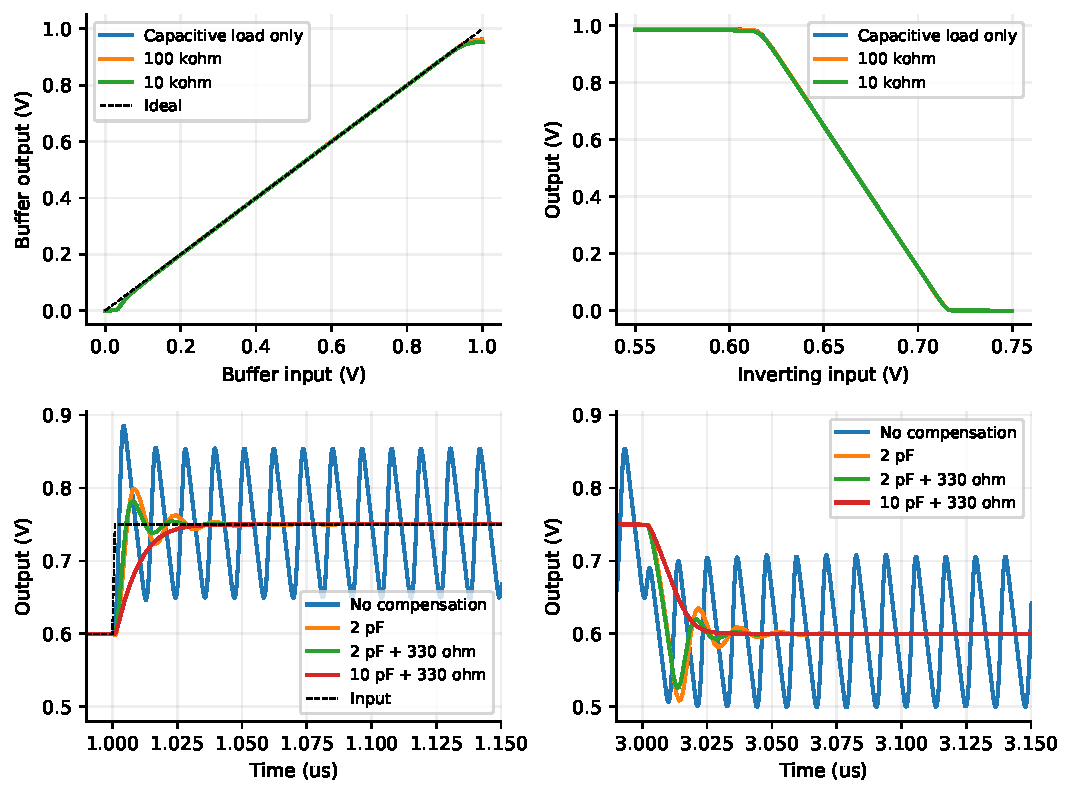
\includegraphics[width=\linewidth]{figures/closed_loop.pdf}
\caption{DC buffer/inverting transfer and local rising/falling step views. The full 5 microsecond observation remains in the CSV data.}
\end{figure}
SR is in V/$\mu$s and denotes the 20--80\% average for this step, not a universal maximum slew rate. A dash means no valid crossing or no settling within the window. Uncompensated falling output is already oscillatory and does not define a clean monotonic slew. The 10 pF + 330 $\Omega$ case settles in 33.8/27.6 ns for rise/fall, with both overshoots below 0.001\%.

\section{Discussion}
The CS second stage adds voltage gain but also an output pole and inversion. Replacing it with a source follower lowers output impedance and improves drive, but its near-unity gain reduces total open-loop gain. Cascoding can increase gain while consuming swing and common-mode headroom. Any topology change requires rechecking feedback polarity and full loop gain; this PM cannot be reused.

PM measures phase distance to the instability condition at unity loop gain, not stability under every load or nonlinear state. Miller compensation splits poles and lowers the dominant pole, usually trading unity bandwidth for PM. A series resistor changes the feed-forward zero. The 2 pF case fails to reproduce the handout's approximately 55 degrees, so it is retained and the 10 pF design is explicitly separate. Page 54 calls -3 dB half amplitude; this report uses $1/\sqrt2$ amplitude, whereas half amplitude is about -6.02 dB. For the uncompensated multipole circuit, $A_0f_{3dB}$ is about 1.42 GHz while the actual unity crossing is 124.56 MHz; they are not interchangeable GBW measures.

\section{Conclusion}
Both Lab 5.A/B circuits and all measurements are complete. Original 2 pF compensation misses 45 degrees. The separate 10 pF + 330 ohm adaptation reaches 80.59 degrees at nominal 10 pF load and settles in both directions. Corner, mismatch, layout and silicon validation are outside these results.

